% \chapter{Fatigue} \label{sec:Fatigue}

\newpage

\def\l{l}
\def\ltilde{\tilde{l}}
\def\gammaMax{\gamma_0}
\def\lw{l_w}
\def\Origin{\mathbb{G}_{xy}(\bm{0})}
\def\Norm{||\mathbb{G}_{xy}||_2}


\section{Introduction}
For a system that oscillates for a long period of time $c^*$ before yielding or absorbing, we find that a large portion of that time is spent with a single oscillator oscillating backwards and forwards, yielding on every half cycle. 


We will begin by defining some concepts which motivate the later discussion.

\subsection{Concept 1 - Local strain}
Every element in our elastoplastic model has a local strain $l$. Following the idea of Picard \etal \cite{picard_elastic_2004}, we will decompose this strain into three components,
\begin{equation}
    \l = \epsilon^{el} + \epsilon^{pl} + \gamma.
\end{equation}
$\epsilon^{el}$ denotes the local elastic strain, $\epsilon^{pl}$ the local plastic strain, which covers the strain lost due to yielding, and $\gamma$, which is the globally applied macroscopic strain. At any step, we know the imposed $\gamma$ and can measure $\ltilde = \epsilon^{el} + \epsilon^{pl}$. Conceptually, $\ltilde$ is a measure of the deviation of an element strain $l$ from the global strain $\gamma$. From the initial configuration, $\ltilde$ changes only due to yielding events, either by itself yielding or through the propagation of stress from another element yielding.

\subsection{Concept 2 - Oscillatory shear}
We are looking at fatigue quasi-static oscillatory shear. This means the globally applied strain $\gamma$ osculates between $\gammaMax$ and $-\gammaMax$ at a rate $\dot{\gamma} \ll 1$. We refer to a full cycle as $\gamma$ starting at $0$, increasing to $\gammaMax$, decreasing to $-\gammaMax$ and returning to $0$. Alternatively, $\gamma$ could first decrease to $-\gammaMax$, increase to $\gammaMax$ and return to $0$; however, by symmetry,  all arguments will still hold. We plot an example cycle in \cref{fig:SineWave}. 

\begin{figure}[hbt]
    \centering
    \includegraphics[width=0.9\linewidth]{chapters/Fatigue/RandomWalk/SineWave.tikz}
    \caption{Plot of one cycle of oscillatory shear. The shaded regions mark the areas of the cycle in which elements can yield.}
    \label{fig:SineWave}
\end{figure}

While our simulation does not involve time due to its quasi-static assumptions, we consider the evolution as a function of cycle $c$. Therefore, $c=1/4$ corresponds to the points where $\gamma=\gammaMax$, $c=1/2$ to $\gamma=0$ (on the way to $-\gammaMax$), $c=3/4$ to $\gamma=-\gammaMax$ and $c=1$ to $\gamma=0$ the starting point. We divide the cycle into four regions:
\begin{enumerate}
    \item Starting at $\gamma=0$, the system is strained in the positive direction until it reaches $\gamma=\gammaMax$. Elements whose absolute local strain $|l|$ exceeds the yield threshold $l_y=1$.
    \item With $\gamma=\gamma_0$ and all yielding occurred, the system starts globally straining back towards $0$. Little to no yielding occurs during this region as all values of $l$ strictly decrease with $\gamma$. Elements are only able to yield in this region if $\ltilde > 1$.
    \item Similarly to region 1, the system is strained towards $-\gammaMax$, with elements whose absolute local strain $|l|$ exceeds $l_y$ yield towards $0$.
    \item Identical behaviour to region 2 with all strains, global and local, increasing until $\gamma=0$.
\end{enumerate}

In regions two and four, we make the statement that little to no yielding occurs, while it is possible that an element could have a value of $|\ltilde| \geq |l_y|$ large enough that it yields at a strain $\gamma$ of the opposite sign. This is highly unlikely and could only occur as a result of a significant amount of stress propagation (like that would occur in a shear band) or the rare event that a sample from the post hop distribution $\mathcal{N}(0, \lw)$ obtains a significantly large value from the origin $\sim 1/\Origin$. 

\subsection{Concept 3 - Yielding}
When an element's stress energy $\tfrac{\mu}{2}l^2$ becomes too large, the element is assumed to yield, propagating its stress to neighbouring elements. We will refer to the threshold energy as $E_y$. In our system, we will take units where $E_y=0.5$ and $\mu=1$. This corresponds to setting the yield threshold for the local strain $l$ to $\pm 1$, or as stated in Concept 2, $|l| \geq 1$. To be specific, elements yield if either their local strain is greater than $1$ or less than $-1$.

When any element yields, it adopts a new local strain
chosen at random from a Gaussian distribution $\lw$. This yielding corresponds to a local plastic yielding event in the material, for example, a sudden rearrangement of a few particles. After such a yielding events the lattice will not be divergence free (force balance is violated). We immediately after yielding reimpose force balance via the Eshelby stress propagator \cite{picard_elastic_2004,eshelby_determination_1997}. The resultant correction to the stress field in Fourier space is therefore,
\begin{equation}
    \hat{\sigma}_{xy}^1 = \mu \hat{\mathbb{ G }}_{ xy } \hat{\epsilon}_{x y}^{\mathrm{pl1}}
\end{equation}
where $\hat{\epsilon}_{x y}^{\mathrm{pl1}}$ is stress drop field in Fourier space and
\begin{equation}
    \hat{\mathbb{ G }}_{ xy } = -4 \frac{ k_x^2 k_y^2 }{ k^4 }
\end{equation}
is the Eshelby stress propagator. The propagator $\hat{\mathbb{ G }}_{ xy }$ is only defined up to a constant due to the singularity at $\bm{k}=\bm{0}$. In practice, this constant is defined by the boundary conditions of the system, where, in a strain-controlled regime, the elastic strain in the system is conserved. As such, the singularity at $\bm{k}=\bm{0}$ is resolved by setting $\hat{\mathbb{G}}_{xy}(\bm{0}) = -1$ such that the total stress lost in the system due to plastic events is $\mu\int d\bm{r}^\prime \epsilon_{x}^{\mathrm{pl1}}(\bm{r}^\prime)$. 

\begin{figure}[hbt]
    \centering
    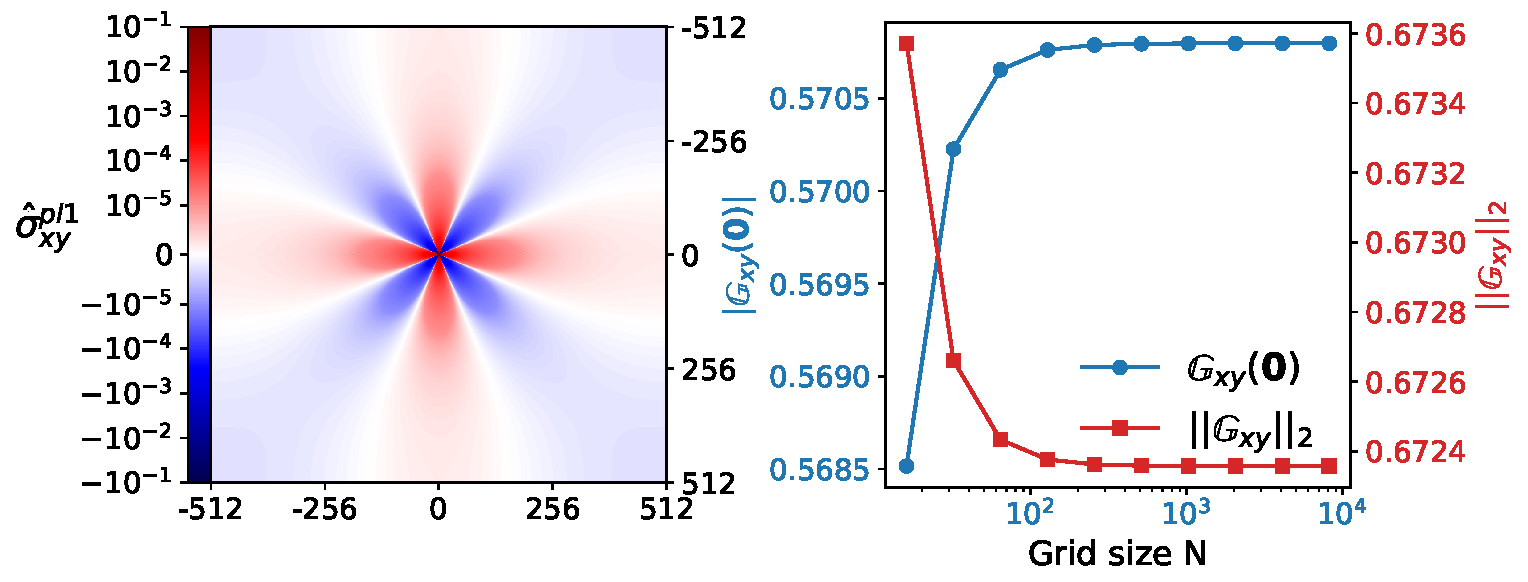
\includegraphics[width=0.9\linewidth]{chapters/Fatigue/RandomWalk/Prop.pdf}
    \caption{{\bf left)} Example propagator yielding from 1 to 0 at $N=1024$. {\bf Right)} Convergence of two important parameters from $\mathbb{G}_{xy}$. The value at the origin $\Origin$ and norm $\Norm$.}
    % \label{fig:Propogator}
\end{figure}

We show an example of the propagator in \cref{fig:Propogator}. Of particular importance are two properties of $\mathbb{G}_{xy}$, the value at the yielding element $\Origin \approx 0.5707$ and the 2-norm $\Norm \approx 0.6724$. These two values do depend on $N$, although they both quickly converge for $N>128$. While $\mathbb{G}_{xy}$ is well defined in Fourier space, the author does not know of any closed analytical forms of these two values. 

\subsection{Concept 4 - Initial Distribution}
The initial distribution of local strains $l$ in the system is drawn from a Gaussian distribution of mean $0$ and standard deviation $l_0$. This random seeding does not naturally obey force balance. Consequently, force balance is immediately imposed through the Eshelby propagator. This has the consequence of reducing the standard deviation of the initial by a factor of $\Norm\approx0.6724$.

\subsection{Concept 5 - End-states}
We are going to classify the final state of our system into two major categories. These two states are mutually exclusive and can be defined as follows:
\begin{itemize}
    \item {\bf Yielded –} We classify a system as yielded following the approach of Pollard \etal \cite{pollard_yielding_2022}. Yielding is detected as a dramatic drop in the system's stress at a fixed $\gamma$, which corresponds to the formation of a shear band within the system. Systems which have undergone the formation of this shear band are classified as yielded.
    \item {\bf Absorbed –} Absorbed states correspond to non-yielded configurations whose distribution $\rho(\tilde l)$ is sufficiently narrow around $0$ that the application of shear causes no further elements to yield. As a result, the distribution no longer evolves under subsequent oscillations.
\end{itemize}
The parameter of interest to this work is $c^*$, which corresponds to the number of cycles to reach an end-state, either yielding or absorbing.

\section{A Simple Picture of the First Cycle} \label{sec:simpleFirstCycle}

\begin{figure}[hbtp]
    \centering
    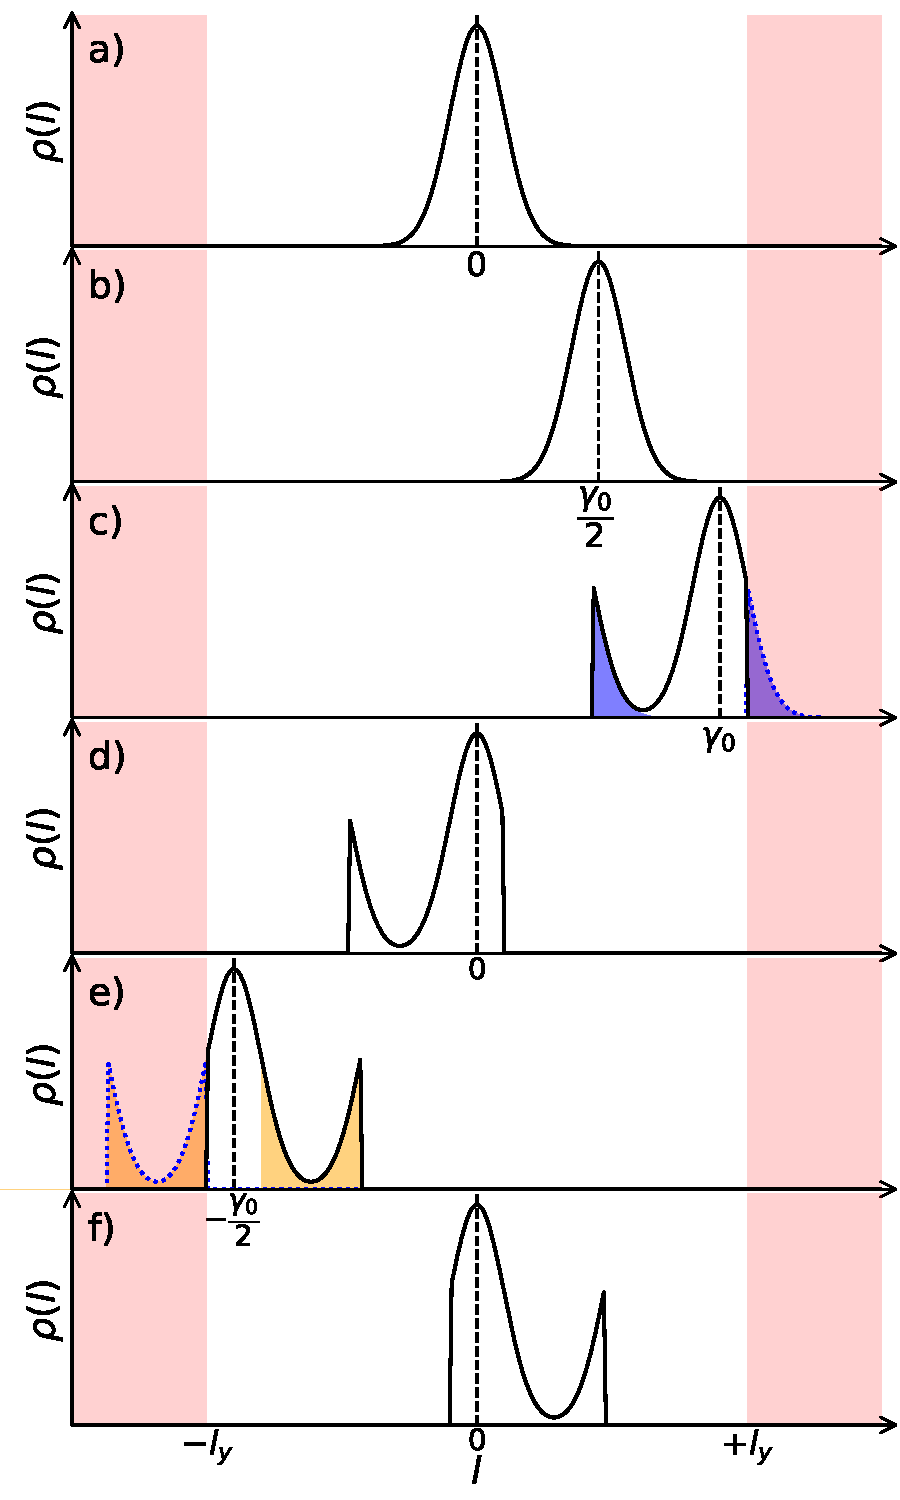
\includegraphics[width=0.8\linewidth]{chapters/Fatigue/RandomWalk/SimpleFirstCycle.pdf}
    \caption{Illustration of how the distribution of $l$ changes in the first cycle. We display the distribution for several key points in the cycle a)-f).}
    \label{fig:SimpleFirstCycle}
\end{figure}

To explore alternative approaches to modelling the system’s physics, we first consider a simplified version of the problem to build intuition for how the distribution of element strains evolves, both over a single cycle and across multiple cycles. In \cref{fig:SimpleFirstCycle} we plot the evolution of the strain distribution over the first cycle, from its initial distribution shown in panel {\bf a} to its state at the end of the cycle in panel {\bf f}. Each subplot shows an idealised point within the cycle, progressing from top to bottom. The distribution at each stage is described as follows:
\begin{enumerate}[label=\textbf{\alph*)}]
    \item $c=0$: The system begins with a narrow Gaussian distribution. As discussed in Concept 4, this distribution has a mean $\mu=0$ and standard deviation $\sigma=l_0\Norm$.
    \item $c=0.083$: the system begins to strain, here in the positive direction, shown at $\gamma=\gammaMax/2$. Since all elements are strained uniformly by $\gamma$, this shifts the mean of the distribution to $\gamma$ without distorting its shape. For such a narrow distribution, few elements have strains $l$ that exceed the yield threshold $l_y$, and the distribution therefore remains essentially unchanged.
    \item $c=0.25$: The system has reached its maximum positive strain $\gamma=\gammaMax$. At this point, a visible fraction of the elements have exceeded the yield threshold and have therefore yielded. This forces the right-hand side of the normal distribution, shown in blue, to translate independently of the bulk behaviour by a factor $-\Origin$. For simplicity, we assume that each element yields to $0$ (the post-hop distribution has the form $\mathcal{N}(0,0)$) before force balance is imposed, and elements do not redistribute this lost stress to neighbouring elements. Of course, this is not the real physics, and we will discuss the impact of these effects later; neglecting them simplifies the present discussion. 
    \item $c=0.5$: After all yielding has occurred at $\gamma=\gammaMax$ all elements have strains $l<l_y$. The system globally strains back to $\gamma=0$, which again now shifts the whole distribution uniformly.
    \item $c=0.75$: We plot the system at its maximum negative strain $\gamma=-\gammaMax$. Again as in {\bf c)}, a large portion of elements have passed the yield threshold, this time $-l_y$, this time shown in orange. These yielding elements include both elements whose initial $l$ value was sufficiently negative and some of the elements that have already yielded during the positive part of the cycle. We plot here with a dotted line the distribution of elements that had not yielded and coloured in yellow the part $\rho(l)$. 
    \item $c=1$: The system is macroscopically strained back to $\gamma=0$. This reveals the now asymmetric distribution $\rho(l)$, which is strongly weighted to positive values and truncated on the right-hand side.  
\end{enumerate}

Following the same assumptions, subsequent cycles follow the same principles, and the system oscillates every half cycle between the distributions presented in {\bf d} and {\bf f}. We make this statement stroboscopically, looking at the distribution only when $\gamma=0$ at $c=n/2$ for $n=0,1,2,3,...$. During phases where the strain is increasing/decreasing towards $\gammaMax$/$-\gammaMax$ (regions 1 and 2 in \cref{fig:SineWave}), elements yield immediately when $|l| \geq l_y$ and as such the distribution transitions gradually between the two states. When an element yields, its strain is reduced by an amount $\Origin$, equal to the width of the truncated distribution (the origin of this is discussed later). Consequently, an element yielding at the rightmost edge of the distribution reappears at the leftmost edge, and vice versa for yielding in the negative direction.

\begin{figure}[hbt]
    \centering
    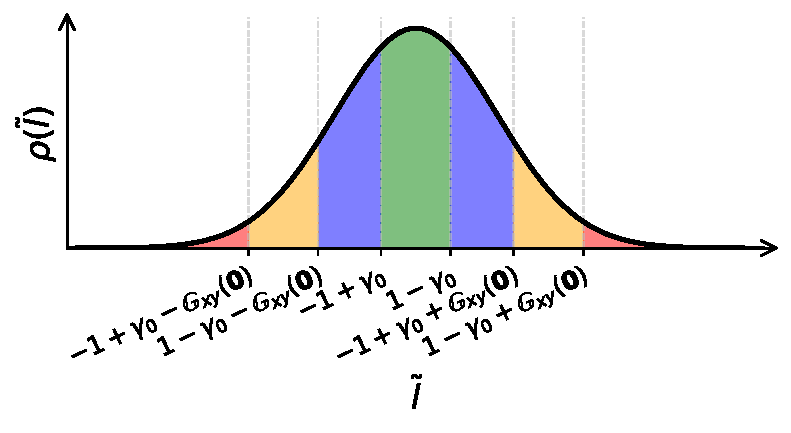
\includegraphics[width=0.95\linewidth]{chapters/Fatigue/RandomWalk/YieldRegions.pdf}
    \caption{A plot of distinct yielding regions for an arbitrary distribution $\rho(\ltilde)$. The green region highlights the absorbed elements which are unable to be strained enough to yield. Elements in the blue regions can yield and map to each other; an element yielding from the positive blue region will lose enough stress to appear in the negative blue region. Elements which yield from the yellow regions enter the green absorbed region.  Elements in the red region have sufficiently large $|\tilde l|$ to yield twice within half a strain cycle; these elements continue yielding until they end up in a blue or red region.}
    \label{fig:YieldRegions}
\end{figure}

Since yielding alters only the element's local elastic strain $\epsilon^{el}$ and plastic strain $\epsilon^{pl}$, and not the global strain $\gamma$, for the simplified case being considered, there exists a 1-1 mapping for $\ltilde$ pre-yielding to $\ltilde$ post-yielding. In \cref{fig:YieldRegions}, we highlight the regions of $\tilde l$ in which elements differ in their post-yield location. For the discussion that follows, we assume $|\gammaMax| < |l_y|$, so that a portion of the distribution (the green region in \cref{fig:YieldRegions}) contains elements that cannot yield. These elements have a $\ltilde$ close enough to $0$ that $|\ltilde + \gammaMax| < |l_y|$, and as such are unable to yield by elastic straining alone. If all elements enter this regime, no further yielding can occur, and we classify the end-state of the system as absorbed.

When an element yield its strain $l$ decreases towards $0$ by a factor of $\Origin$. Elements whose $\ltilde$ lie in the blue regions when yielding will decay to the other blue region. These elements will go on to yield in the next half cycle and continue to oscillate between the two blue regions. Conversely, elements in the yellow regions that undergo a yielding event have a post-yield $\ltilde$ that lies in the green region and, as such, become absorbed for subsequent cycles.

Elements which yield in the red regions have large enough $\ltilde$ to yield at least twice in a single strain cycle. These elements strain decay towards $0$ with each subsequent yielding event until their $\ltilde$ lies in either the blue or yellow region and follows the respective behaviour described above.  
A natural consequence of this behaviour is that the truncated distribution, when measured stroboscopically at $\gamma=0$,  has a width equal to $\Origin$. After the first cycle, all elements must exist in either the blue or green region, as yielding in any other region decays to these regions. At each of these points, elements only exist in one of the two blue regions, the positive blue region at the start of each cycle and the negative blue region at the midpoint of each cycle. This gives the distribution at these points an overall width of $\Origin$.

\section{The Effect of $\lw$}

In the discussions so far, we have considered a simple model whereby when an element yields, it resets its $l$ to 0, before force balance is reimposed, so all elements lose exactly $\Origin$ strain. This makes a trivial system, as an element exists in either the green or blue regions and remains there indefinitely, with the distribution returning to the same configuration at the start of each cycle. 

\begin{figure}[hbt]
    \centering
    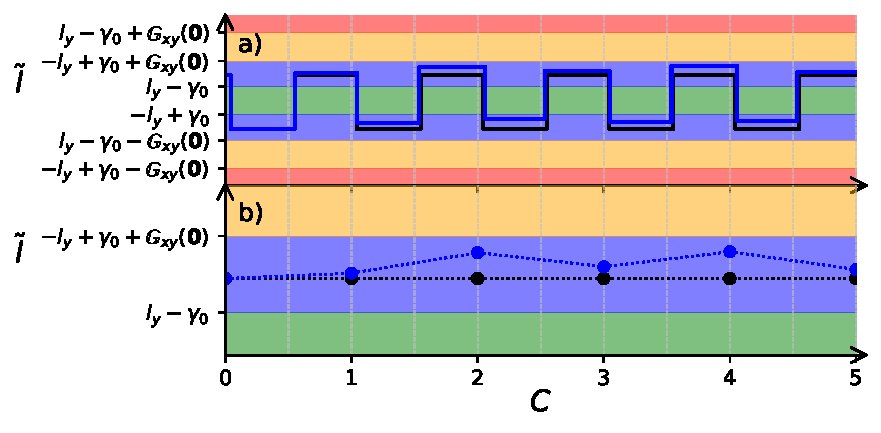
\includegraphics[width=0.95\linewidth]{chapters/Fatigue/RandomWalk/OscillatorRegions.pdf}
    \caption{An illustration of a single element yielding. In black we plot the trivial cases where each element yields to $0$, before restoring force balance. The blue line illustrates a case where, when an element yields, it instead resets its strain to a new local strain chosen at random from a Gaussian distribution $\lw$. {\bf a)} plots $\ltilde$ for a single element in both cases across the first five cycles. {\bf b)} extracts $\ltilde$ stroboscopically at the start of each cycle. Dotted lines are there to guide the eye and do not represent the actual trends in $\ltilde$.}
    \label{fig:OscillatorRegions}
\end{figure}

However, as stated in Concept 3, when an element yields, it instead resets its strain to a new local strain chosen at random from a Gaussian distribution $\lw$. In \cref{fig:OscillatorRegions}, we illustrate the effect of this. In {\bf a)} we plot $\ltilde$ throughout the cycle, each element yields twice, one in each half cycle, oscillating between positive and negative values. In black, we plot the trivial case where $\lw=0$, $\ltilde$ osculates between two values, returning to the same value at the start of each cycle as shown in {\bf b)}. Instead, when we introduce the post-hop distribution, each element instead loses $\pm (1+\mathcal{N}(0,\lw))\Origin$. As a result, when observed stroboscopically at the start of each cycle, the element appears to randomly walk.

\begin{figure}[hbt]
    \centering
    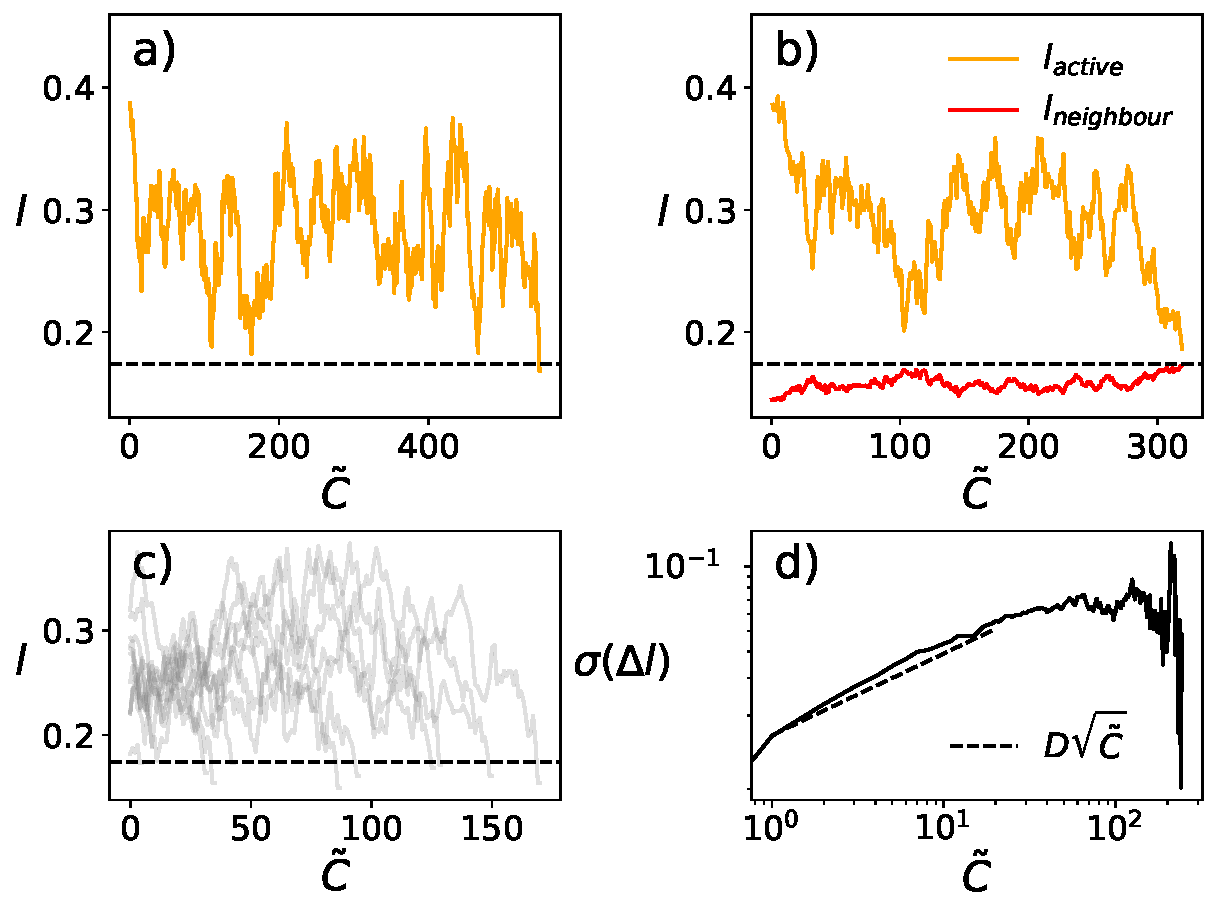
\includegraphics[width=0.9\linewidth]{chapters/Fatigue/RandomWalk/RandomWalks.pdf}
    \caption{Random walks observed in Elasto-plastic simulations. {\bf a)} Blue like plots a random walk observed for the last element in a system which ends up absorbing. {\bf b)} A pair of random walks in a yielding system. The blue element oscillates as a result of the post-hop yielding. This is coupled to the absorbed orange element through stress propagation, resulting in it leaving the absorbed region. {\bf c)} A collection of random walks across many systems. {\bf d)} The standard deviation of the displacement of each random walk.}
    \label{fig:RandomWalks}
\end{figure}

When yielding from a positive value, an element's $\ltilde$ decreases by a factor $(1+\mathcal{N}(0,\lw))\Origin$, on the next half cycle, when yielding from a negative value, $\ltilde$ gains $(1+\mathcal{N}(0,\lw))\Origin$. The resulting change in $\ltilde$ after a full cycle is therefore $(\mathcal{N}(0,\lw) + \mathcal{N}(0,\lw))\Origin$. As each sample of $\mathcal{N}(0,\lw)$ is independent, the resultant distribution has the $\mathcal{N}(0,\sqrt{2}\lw)\Origin$ or $\mathcal{N}(0,\sqrt{2}\Origin\lw)$. We illustrate some examples of this random walk in blue in \cref{fig:RandomWalks}{\bf a)-b)} and grey in {\bf c)}. A common way to verify a random walk is to consider the variance of the displacement of each random walk $\Delta \ltilde(\tilde{c}) = \ltilde(\tilde{c}) - \ltilde(0)$ where $\tilde{c}$ tracked the number of cycles from the start of the random walk, over many such walks. We plot this \cref{fig:RandomWalks}d) where for small $\tilde{c}$, where we have enough samples, the variance tracks our analytical result.

\section{Stress Propagation}
The second concept introduced in Concept 3 is that of stress propagation. When an element yields and a force balance is imposed, it redistributes some of its stress (we have taken units where $\mu=1$ so stress and strain are equivalent in this context) to neighbouring elements. Consequently, all neighbouring elements $\ltilde$ are affected by an element yielding. This phenomenon is illustrated in \cref{fig:RandomWalks}b) where the oscillating element, shown in blue, causes a scaled random walk with variance $\sqrt{2}\mathbb{G}_{xy}(\bm{r})\lw$ for a cell at position $\bm{r}$ relative to an element yielding at $\bm{0}$. We highlight this example because the orange element lies in the absorbed region and, due to oscillations of the blue element, can escape it, ultimately leading to material failure. The boundary between the green and blue regions is marked here in red. In addition to elements being able to leave the absorbed region, stress propagation can also push elements that lie on the boundary into the absorbed region.

\section{A Division of \quotes{Timescales}}
Motivated by the discussion above and the data presented in \cref{fig:1Osc}, we aim to divide the time it takes for a system to yield or absorb $c^*$ into two components. In \cref{fig:1Osc} we see that systems that have fewer oscillating elements towards the end of their lifespan take longer to reach their end state. We expect this simply comes from the lack of activity in the system, when there is only one element oscillating in the system, all elements do a trivial random walk proportional to $\lw$. When there are multiple elements oscillating, each element has more chances to change its $\ltilde$, and as a result are more likely to end up in the absorbed region or reach a configuration where a shear band forms. 

\begin{figure}[hbt]
    \centering
    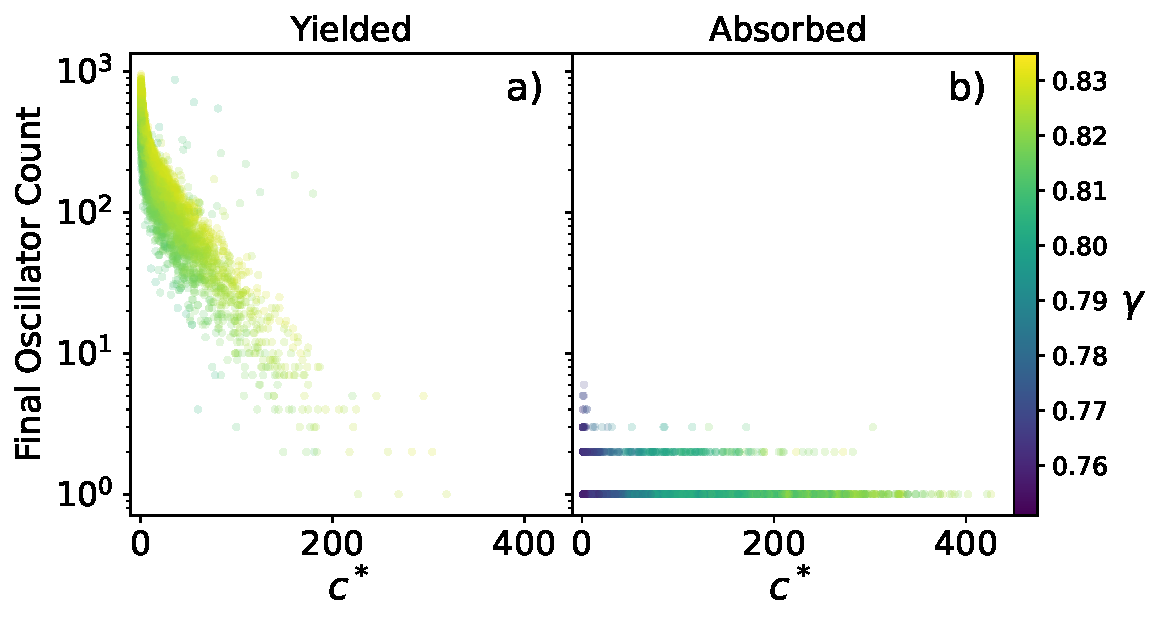
\includegraphics[width=0.9\linewidth]{chapters/Fatigue/RandomWalk/1Osc.pdf}
    \caption{The final number of elements left in the oscillating just before the system reaches its end-state. We plot a sample of cases for when the system {\bf a)} yields or {\bf b)} absorbs. Data is plotted for $l_0=0.075$, $\lw=0.02$ and $N=1024$. }
    \label{fig:1Osc}
\end{figure}

We therefore will divide $c^*$ into two time scales, the time it takes to reach a single oscillator in the system $c^* - \tilde{c}$ and the time the system exists with a single oscillator $\tilde{c}$. We make two observations. First, an element can be pulled out of the absorbed region and begin to oscillate; in almost all cases, this rapidly leads to the formation of a shear band. Second, we currently consider cases in which only a single element oscillates; in sufficiently large systems, however, multiple elements can oscillate \emph{almost} independently ($\mathbb{G}_{xy}(\bm{r}) \sim 0$). Based on the rate of convergence in \cref{fig:Propogator}b) this distance appears to be $\approx 256$, as this is the system size where self-interaction no longer visibly affects $\Norm$ or $\Origin$. This implies that in our systems of size $N=1024$, approximately four such elements could exist independently. For simplicity, and so that we can use the data we have already collected, we consider cases where exactly one element is left and where the final oscillator decays to an absorbed state singularly.

For the moment, we will ignore the time to reach a single oscillator in the system $c^* - \tilde{c}$ as this proves to be the more complicated problem of the two. Instead, we will first focus on solving the second problem, the number of cycles $\tilde{c}$ a single element randomly walks when it is the last element remaining. We will also pose the problem only for absorbing states for the moment, as in this context, we only need to consider a single element. We hope that the insights into this case will allow us to gain insight into systems which ultimately yield.

\section{Modelling $\tilde{c}$}

Considering the random walk exhibited by $\ltilde$ when observed stroboscopically at the end of each full cycle (shown in \cref{fig:OscillatorRegions}b), the walk terminates when $\ltilde$ enters the absorbed (green) region. We can therefore formulate this as a first-passage time problem \cite{Redner_2001}, where $\tilde{c}$ is the first cycle at which the random walk enters the absorbed region. The appropriate first-passage formulation then depends on the geometry of the absorbed region: while the green region shares a single boundary with the active blue regions, we hypothesise that the element can be absorbed at both boundaries. Elements which lie close to the positive green-blue boundary may yield and end up, due to the post-hop distribution, in the negative yellow region. During the subsequent half-cycle, such elements will yield again into the green region, unless the second post-hop sample returns them to the active (blue) region. Elements close to the (positive) blue-yellow boundary may directly yield to the absorbed region.

While this sequence of steps may appear complicated, from the perspective of the stroboscopic random walk, elements can be absorbed at both boundaries. In \cref{fig:rho(l)_examples} we plot the probability density of $\ltilde_0$, the initial value of $\ltilde$ for elements that subsequently exhibit a random walk. In both cases, we see a hard boundary at $1-\gammaMax$ (green-blue) and a cut-off at the $-1+\gammaMax+\Origin$ boundary (blue-yellow). Elements can temporarily reside in the yellow region, but have a high probability of yielding into the absorbed region, with this probability increasing with $\ltilde$.

\begin{figure}[hbt]
    \centering
    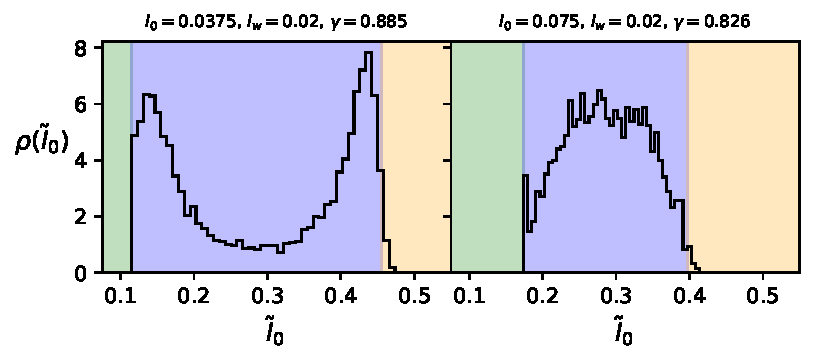
\includegraphics[width=0.9\linewidth]{chapters/Fatigue/RandomWalk/rho(l)_Examples.pdf}
    \caption{Probability density $\rho(\ltilde_0)$ of the initial value $\ltilde_0$ for each random walk. The distributions are constructed from more than 5000 simulations that terminate in a random-walk regime, with $\ltilde_0$ extracted at the end of the first cycle after only one element remains.}
    \label{fig:rho(l)_examples}
\end{figure}

We consider two first-passage time problems. The first has a single absorbing boundary at $1-\gammaMax$, and serves to test whether the assumption of two absorbing boundaries is necessary. The second has two absorbing boundaries, located at the edges of the active (blue) region.

\subsection{One Boundary Condition}
To model the concentration $\rho(\tilde{c})$ in the case of a single absorbing boundary at $\ltilde = 1-\gammaMax$, we consider a first-passage problem on a semi-infinite domain $x>0$ with an absorbing boundary at $x=0$. To the authors’ knowledge, no analytical solution exists for $\rho(\tilde{c})$ for a process with continuous spatial states but discrete time steps. In these cases, it is common to instead consider a continuous-time approximation, which can be modelled as a diffusion process of the form
\begin{equation}
    \frac{\partial c(x, t)}{\partial t} = D \frac{\partial^2 c(x, t)}{\partial x^2}
\end{equation}
where $D$ is a diffusion coefficient and $c(x,t)$ the concentration. We impose an absorbing boundary condition $c(0, t) = 0$. Using the method of images described in Ref.~\cite{Redner_2001}, $c(x, t)$ can be constructed as the sum of a Gaussian and an
anti-Gaussian:
\begin{equation}
    c(x, t|x_0)=\frac{1}{\sqrt{4 \pi D t}} \left[ e^{-(x-x_0)^2/4Dt} - e^{-(x+x_0)^2/4Dt}\right].
\end{equation}
Assuming a particle starts at $x_0>0$, we write the initial distribution as $c(x, 0)=\delta(x-x_0)$. As $c(x, 0)$ is normalised, the first-passage probability $f(t|x_0)$ to the origin at time $t$ is just the flux to this point. Therefore
\begin{equation}
    f(t|x_0) = -D \left. \frac{\partial c(x,t)}{\partial x}\right|_{x=0} = \frac{x_0}{\sqrt{4\pi Dt^3}}e^{-x_0^2/{4Dt}}.
\end{equation}
This distribution is sometimes termed the inverse Gaussian density. 

\subsection{Two Boundary Condition}
The two-boundary solution can be solved similarly. Again, to the author's knowledge, there is no closed solution in the case of continuous spatial states but discrete time steps. As such, a diffusion process is commonly used as an approximation. The diffusion process again takes the form,
\begin{equation}
    \frac{\partial c(x, t)}{\partial t} = D \frac{\partial^2 c(x, t)}{\partial x^2}. \label{eq:2BCDiffusion}
\end{equation}
This time with two boundary conditions $c(0,t)=0$ and $c(L,t)=0$. We assume that particles start at $x_0 \in (0,L)$, such that $c(x, 0)=\delta(x-x_0)$. The solution to \cref{eq:2BCDiffusion} with two absorbing boundary conditions is well known and takes the form
\begin{equation}
    c(x, t| x_0) = \sum_{n=1}^\infty \frac{2}{L} \sin\left( \frac{n \pi x_0}{L} \right) \sin\left( \frac{n \pi x}{L} \right) \exp \left[ -D \left( \frac{n \pi}{L} \right)^2 t\right]
\end{equation}
where the constant factor $\frac{2}{L} \sin\left( \frac{n \pi x_0}{L} \right)$ comes from the initial distribution. Instead of calculating $f(t)$ from the flux crossing each boundary, we instead consider the survival function, which measures the probability that the particle has not yet been absorbed by time $t$.
\begin{align}
    S(t|x_0) &= \int c(x, t| x_0) dx \\
    &= \sum_{n=1}^\infty \frac{2}{n \pi}\sin\left( \frac{n \pi x_0}{L} \right) \left( 1 - (-1)^n\right)\exp \left[ -D \left( \frac{n \pi}{L} \right)^2 t\right].
\end{align}
Only odd terms contribute, so we can write 
\begin{equation}
    S(t|x_0) = \frac{4}{\pi} \sum_{k=1}^\infty \frac{1}{2k+1} \sin\left( \frac{(2k+1) \pi x_0}{L} \right)\exp \left[ -D \left( \frac{(2k+1) \pi}{L} \right)^2 t\right].
\end{equation}
The first passage time density is the amount leaving the system at a time $t$, so
\begin{equation}
    f(t|x_0) = -\frac{\partial S(t|x_0)}{\partial t} = \frac{4D\pi}{L^2} \sum_{k=1}^\infty (2k+1) \sin\left( \frac{(2k+1) \pi x_0}{L} \right)\exp \left[ -D \left( \frac{(2k+1) \pi}{L} \right)^2 t\right].
\end{equation}

\subsection{Combining the Results}
Both first passage time distributions rely on a diffusion approximation for the underlying stochastic evolution of $\tilde{l}$. We therefore first relate the diffusion coefficient $D$ to the discrete random walk observed in the simulations.


For a one-dimensional random walk with independent increments $\xi_n$ of zero mean and variance $\sigma^2$, the mean-square displacement satisfies
\begin{equation}
    \mathbb{E}\left[(X_n - X_0)^2\right] = n \sigma^2 .
\end{equation}
In the continuum limit, the corresponding diffusion process obeys
\begin{equation}
    \mathbb{E}\left[(x(t) - x_0)^2\right] = 2 D t .
\end{equation}
Assuming we want $t=1,2,...$ to correspond with cycles $n=1,2,...$, then matching these expressions yields
\begin{equation}
    D = \frac{\sigma^2}{2} .
\end{equation}

The unconditional distribution $f(t)$ for each case is then obtained by averaging over the distribution of initial positions,
\begin{equation}
    f(t) = \int f(t|x_0)\rho(x_0) dx_0.
\end{equation}
As a starting point, we take the samples shown from \cref{fig:rho(l)_examples} and offset the initial distributions $\ltilde_0$ such that the lower boundary lies at $0$. We plot the resulting distributions in \cref{fig:CtildeBC}. The blue lines, illustrating the model with one boundary condition, diverge quickly from the data taken from the elastoplastic model. In contrast, the two boundary condition model (in red) matches much more closely, particularly at low $\tilde{c}$. 

\begin{figure}[hbt]
    \centering
    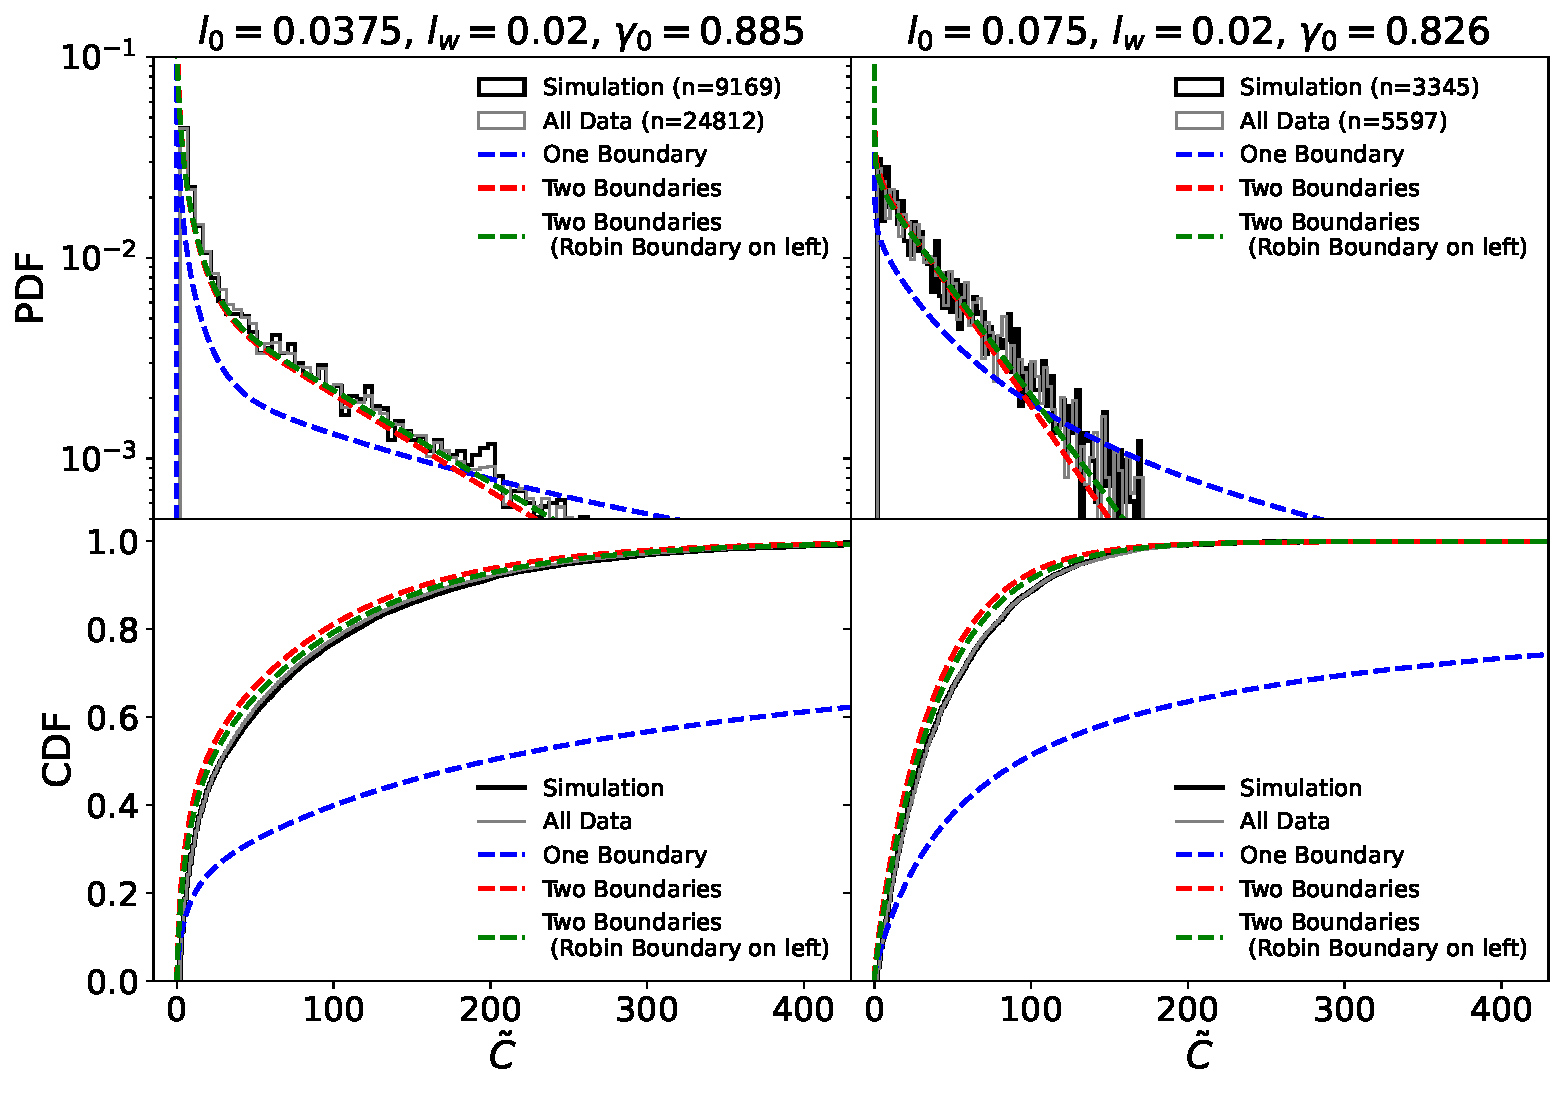
\includegraphics[width=0.9\linewidth]{chapters/Fatigue/RandomWalk/Ctilde_overlays.pdf}
    \caption{Fits of the one- and two-boundary-condition models. We show two datasets from the full elastoplastic simulations: \emph{Simulation}, which corresponds to the subset of runs contributing the initial values $\tilde{\ell}_0$ to the distributions in \cref{fig:rho(l)_examples}, and \emph{All data}, which includes all simulations that resulted in a valid random walk. The two boundary solution takes the first 1000 terms of the Fourier series. We also plot a two-boundary solution with a Robin boundary on the left-hand side with $\kappa$ approximately equivalent to a $50:50$ absorption/reflection chance (solved using a finite difference model).}
    \label{fig:CtildeBC}
\end{figure}

While the two boundary solution matches significantly closer than that of the one boundary model, it still fails to capture the behaviour fully. We expect this due to the incorrect modelling boundary conditions. While the lower boundary has a hard cut-off at $1-\gammaMax$, elements have multiple chances to remain in the system as previously discussed. The upper boundary is not actually a true boundary with elements able to remain above $-1+\gammaMax+\Origin$ for several cycles. However does provide a cleaner condition with elements yielding directly into the absorbed region. We plot a slightly more complicated case solved numerically in green, with a Robin boundary on the left-hand side with $\kappa$ approximately equivalent to a $50:50$ absorption/reflection rate. This matches closer than the true solution, but is still unable to fully capture the whole physics. 

\subsection{From Start to End}
If we assume that the current model is correct, we can think about applying it to the first problem, which is how long it takes to reach a single oscillator. So far, our model does not capture any cooperative effects resulting from stress propagation, which we know if important to the early evolution of the system. As a test, we will continue under this assumption so no propagation. Imagining each element oscillates independently throughout, then can use the same diffusion models we constructed before. 

For notational purposes, we will define 
\begin{itemize}
    \item $c^*$ to be the total lifetime of the material.
    \item $\tilde{c}$ to be the number of cycles at one oscillator as before.
    \item $c^* - \tilde{c}$ to therefore be the number of cycles to reach one oscillator.
    \item $\ltilde_0$ to be $\ltilde$ at $c=0$, the start of the simulation.
    \item $\ltilde_1$ to be $\ltilde$ at $c^* - \tilde{c}$, the cycle at which the system reaches one oscillator. 
\end{itemize}
Therefore we split the problem into two parts, we first solve for $c^* - \tilde{c}$ and find the concentration $c(\ltilde, c^* - \tilde{c})$, the distribution of $\ltilde$ at $c^* - \tilde{c}$, which when normalised becomes initial condition $\rho(\ltilde_1)$ for the second step. Starting from this distribution, we then find the mean exit time $\tilde{c}$.

The time to reach one oscillator $c^* - \tilde{c}$ is equivalent to the time for $S(t)$ to decay such that $S(t) \leq 1/N_xN_y$. The model is initialised with a normalised distribution $\rho(\tilde{l}_0)$ of unit area, representing all $N_xN_y$ elements. Only elements in the regions $(1-\gammaMax, -1+\gammaMax+\Origin)$ and $( 1-\gammaMax-\Origin,-1+\gammaMax)$ are considered activ,e with all other elements being absorbed immediately. We assume that the system undergoes an initial cycle (as described in \cref{sec:simpleFirstCycle}) with elements in the negative region yielding into the positive region. The initial distribution $\rho(\ltilde_0)$ in the region is therefore defined by
\begin{equation}
\rho(\ltilde_0)
= g(\ltilde_0; 0, \Norm l_0) + g(\ltilde_0; \Origin, \Norm l_0),
\qquad
\ltilde_0 \in (1-\gammaMax,\,-1+\gammaMax+\Origin),
\end{equation}
where $g(x;\mu,\sigma)$ is the normal probability density function
\begin{equation}
g(x;\mu,\sigma)
= \frac{1}{\sqrt{2\pi}\sigma}
\exp\left(-\frac{(x-\mu)^2}{2\sigma^2}\right).
\end{equation}
This is equivalent to the region shaded in yellow in \cref{fig:SimpleFirstCycle}e. This distribution is then assumed to decay under a random walk when observed stroboscopically at $c=1,2,3,.....$. The cycle $c^* - \tilde{c}$ can therefore be found by solving,
\begin{equation}
    S(t) = \int S(t|\ltilde_0)\rho(\ltilde_0) d\ltilde_0 = \frac{1}{N_xN_y},
\end{equation}
through a bisection method with a tolerance of $10^{-6}$. We take this to be the mean time to reach one oscillator $\langle c^* - \tilde{c} \rangle$.  

Once this time has been found, the predicted concentration $c(\ltilde_0, c^* - \tilde{c})$ can be found through
\begin{equation}
    c(\ltilde,c^* - \tilde{c}) = \int c(\ltilde,c^* - \tilde{c}|\ltilde_0)\rho(\ltilde_0) d\ltilde_0
\end{equation}
which, when normalised, forms the initial distribution of the single independent random walkers $\rho(\ltilde_1)$. We use the closed form of the mean exit time $\tilde{t}$ for two absorbing boundary conditions
\begin{equation}
    \langle \tilde{t} \rangle = \frac{x(L-x)}{2D},
\end{equation}
and take the average over $\rho(\ltilde_1)$ to get $\tilde{c}$. We plot the results of this model in \cref{fig:TwoStepComp}, comparing the two timescales independently.

\begin{figure}[hbt]
    \centering
    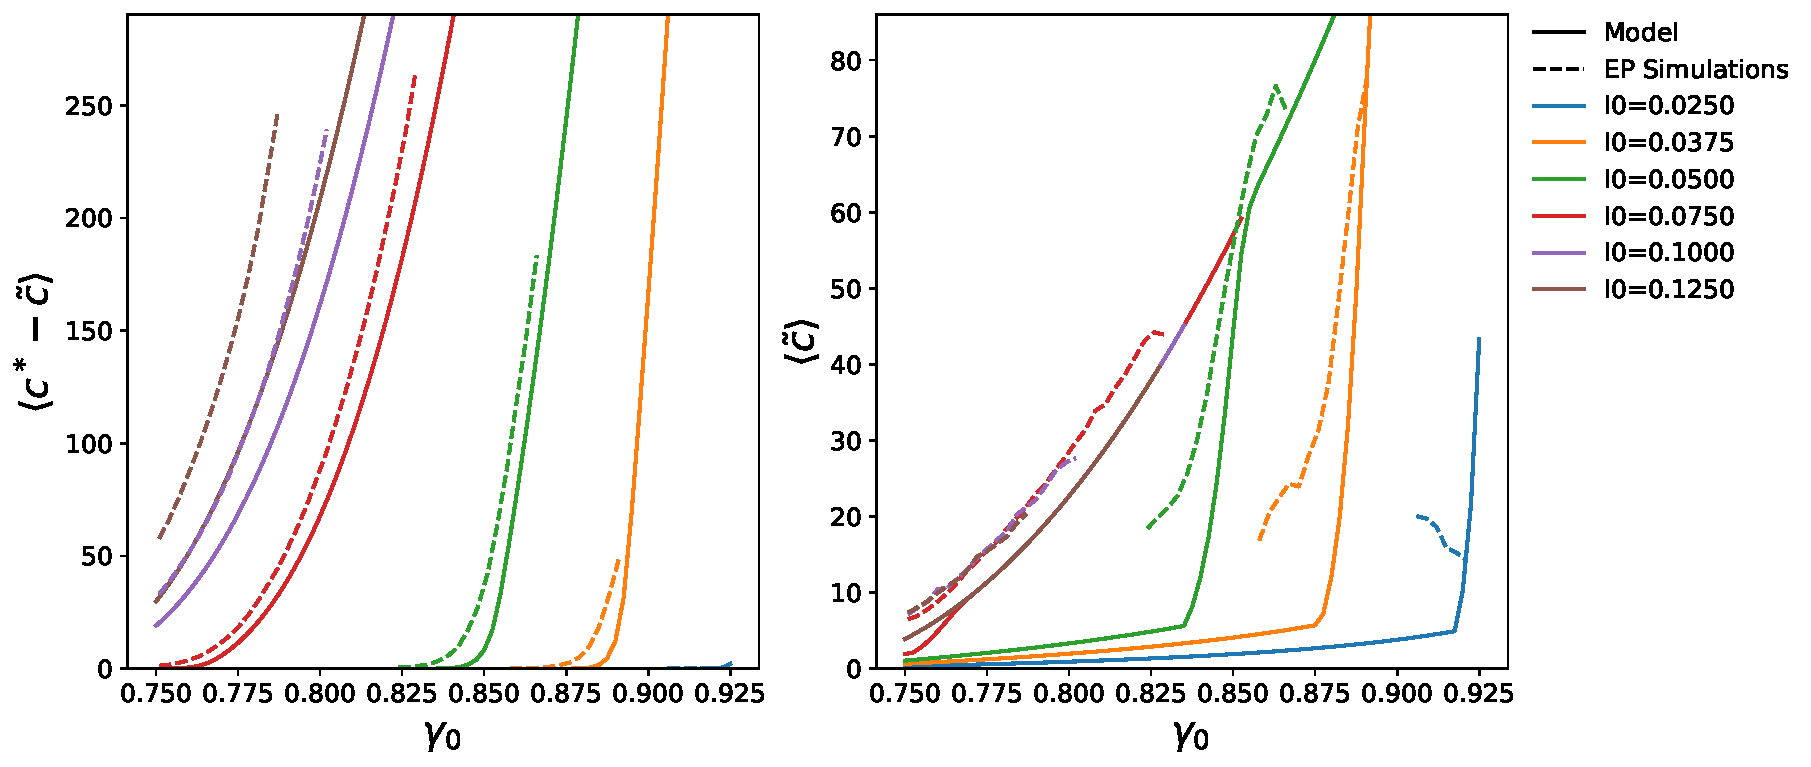
\includegraphics[width=0.9\linewidth]{chapters/Fatigue/RandomWalk/Double_l0_comparison.pdf}
    \caption{Comparison of two timescales taken from numerical data and semi-analytical results.}
    \label{fig:TwoStepComp}
\end{figure}

The overall trends match qualitatively with the curves diverging at around the same parameter ranges. However, in particular, the predictions for $c^* - \tilde{c}$ at high $l_0$ break down quickly. In these regimes, we see more yielding, and as such, the ignored effects start to become important. At a lower $l_0$, we see a closer match, although still predicting delay yielding occurs at a higher $\gammaMax$ than the simulations. The author feels the model captures the behaviour well for $\tilde{c}$ with the non-alignments coming from the bad predictions of $\rho(\ltilde_1)$. We illustrate this hypothesis by overlaying the analytical predictions of $\rho(\ltilde_1)$ over the numerical distribution (already shown in \cref{fig:rho(l)_examples}) in \cref{fig:rho(l)_Comparison}.

\begin{figure}[hbt]
    \centering
    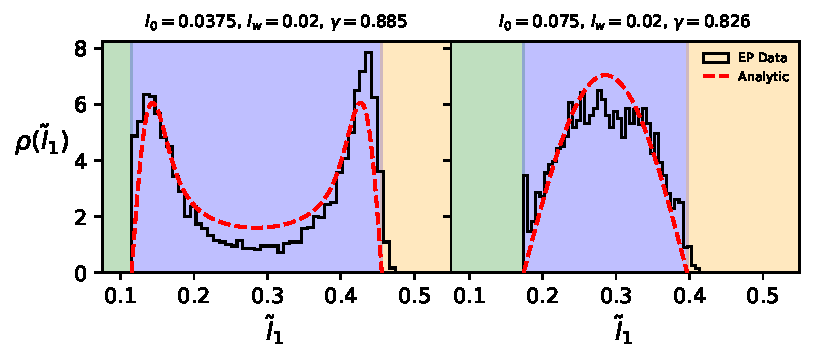
\includegraphics[width=0.9\linewidth]{chapters/Fatigue/RandomWalk/rho(l)_Comparison.pdf}
    \caption{Probability density $\rho(\ltilde_0)$ of the initial value $\ltilde_0$ for each random walk. The distributions are constructed from 2500 simulations that terminate in a random-walk regime, with $\ltilde_1$ extracted at the end of the first cycle after only one element remains. In red we plot the analytical prediction of $\rho(\ltilde_1)$ from our model with two absorbing boundaries.}
    \label{fig:rho(l)_Comparison}
\end{figure}